% HMC Math dept HW template example
% v0.04 by Eric J. Malm, 10 Mar 2005
\documentclass[12pt,letterpaper,boxed,cm]{hmcpset}

% set 1-inch margins in the document
\usepackage[margin=1in]{geometry}
\usepackage{mathtools}
\usepackage{mathrsfs}
% include this if you want to import graphics files with /includegraphics
\usepackage{graphicx}
\usepackage{cases}
\usepackage{hyperref}
\usepackage{siunitx}
\usepackage{tikz}
\usepackage{cases}
\usetikzlibrary{arrows}

% info for header block in upper right hand corner
\name{Name: ~~~~~~~~~~~~~~~~~~~~~~~~~~~~~~~}
\class{Physics 51}
\assignment{Homework \#14}
\duedate{October 27, 2016}

\newcommand{\ev}[2]{\Big|_{#1}^{#2}}
\newcommand{\evv}[2]{\Big|_{#1}^{#2}}
\newcommand{\set}[1]{\left\{#1\right\}}
\newcommand{\s}[1]{\sqrt{#1}}
\newcommand{\f}[2]{\frac{#1}{#2}}
\newcommand{\p}[2]{\frac{\partial #1}{\partial #2}}
\providecommand{\t}[1]{\text{#1}}
\providecommand{\span}[1]{\text{span}\left(#1\right)}
\providecommand{\set}[1]{\left\{#1\right\}}
\providecommand{\l}[0]{\left}
\providecommand{\r}[0]{\right}
\newcommand{\m}[1]{\begin{matrix}#1\end{matrix}}
\newcommand{\bm}[1]{\begin{bmatrix}#1\end{bmatrix}}
\renewcommand{\bf}[1]{\mathbf{#1}}
\newcommand{\pn}[1]{\left( #1 \right)}
\newcommand{\abs}[1]{\left| #1 \right|}
\newcommand{\bk}[1]{\left[ #1 \right]}
\newcommand{\cis}[1]{\pn{\cos\pn{#1} + i\sin\pn{#1}}}
\newcommand{\cisi}[1]{\pn{\cos\pn{#1} - i\sin\pn{#1}}}
\renewcommand{\Im}[1]{\text{Im}\pn{#1}}
\renewcommand{\Re}[1]{\text{Re}\pn{#1}}
\renewcommand{\k}[0]{\f{1}{4\pi\epsilon_0}}
\renewcommand{\part}[1]{\vspace{1em}\noindent(#1)}

\makeatletter
\renewcommand*\env@matrix[1][*\c@MaxMatrixCols c]{%
  \hskip -\arraycolsep
  \let\@ifnextchar\new@ifnextchar
  \array{#1}}
\makeatother
\begin{document}
\problemlist{36-E21, 36-P9}


\begin{problem}[36-E21]
	In the circuit shown in Fig. 36-20, $\varepsilon = \SI{10}{V}$, $R_1 = \SI{5.0}{\ohm}$, $R_2 = \SI{10}{\ohm}$, and $L = \SI{5.0}{H}$. For the two separate conditions (I) switch S just closed and (II) switch S closed for a long time, calculate
	\begin{enumerate}
		\item[(a)] the current $i_1$ through $R_1$,
		\item[(b)] the current $i_2$ through $R_2$,
		\item[(c)] the current $i$ through the switch,
		\item[(d)] the potential difference across $R_2$,
		\item[(e)] the potential difference across $L$, and
		\item[(f)] $\f{di_2}{dt}$.
	\end{enumerate}
	\begin{center}
		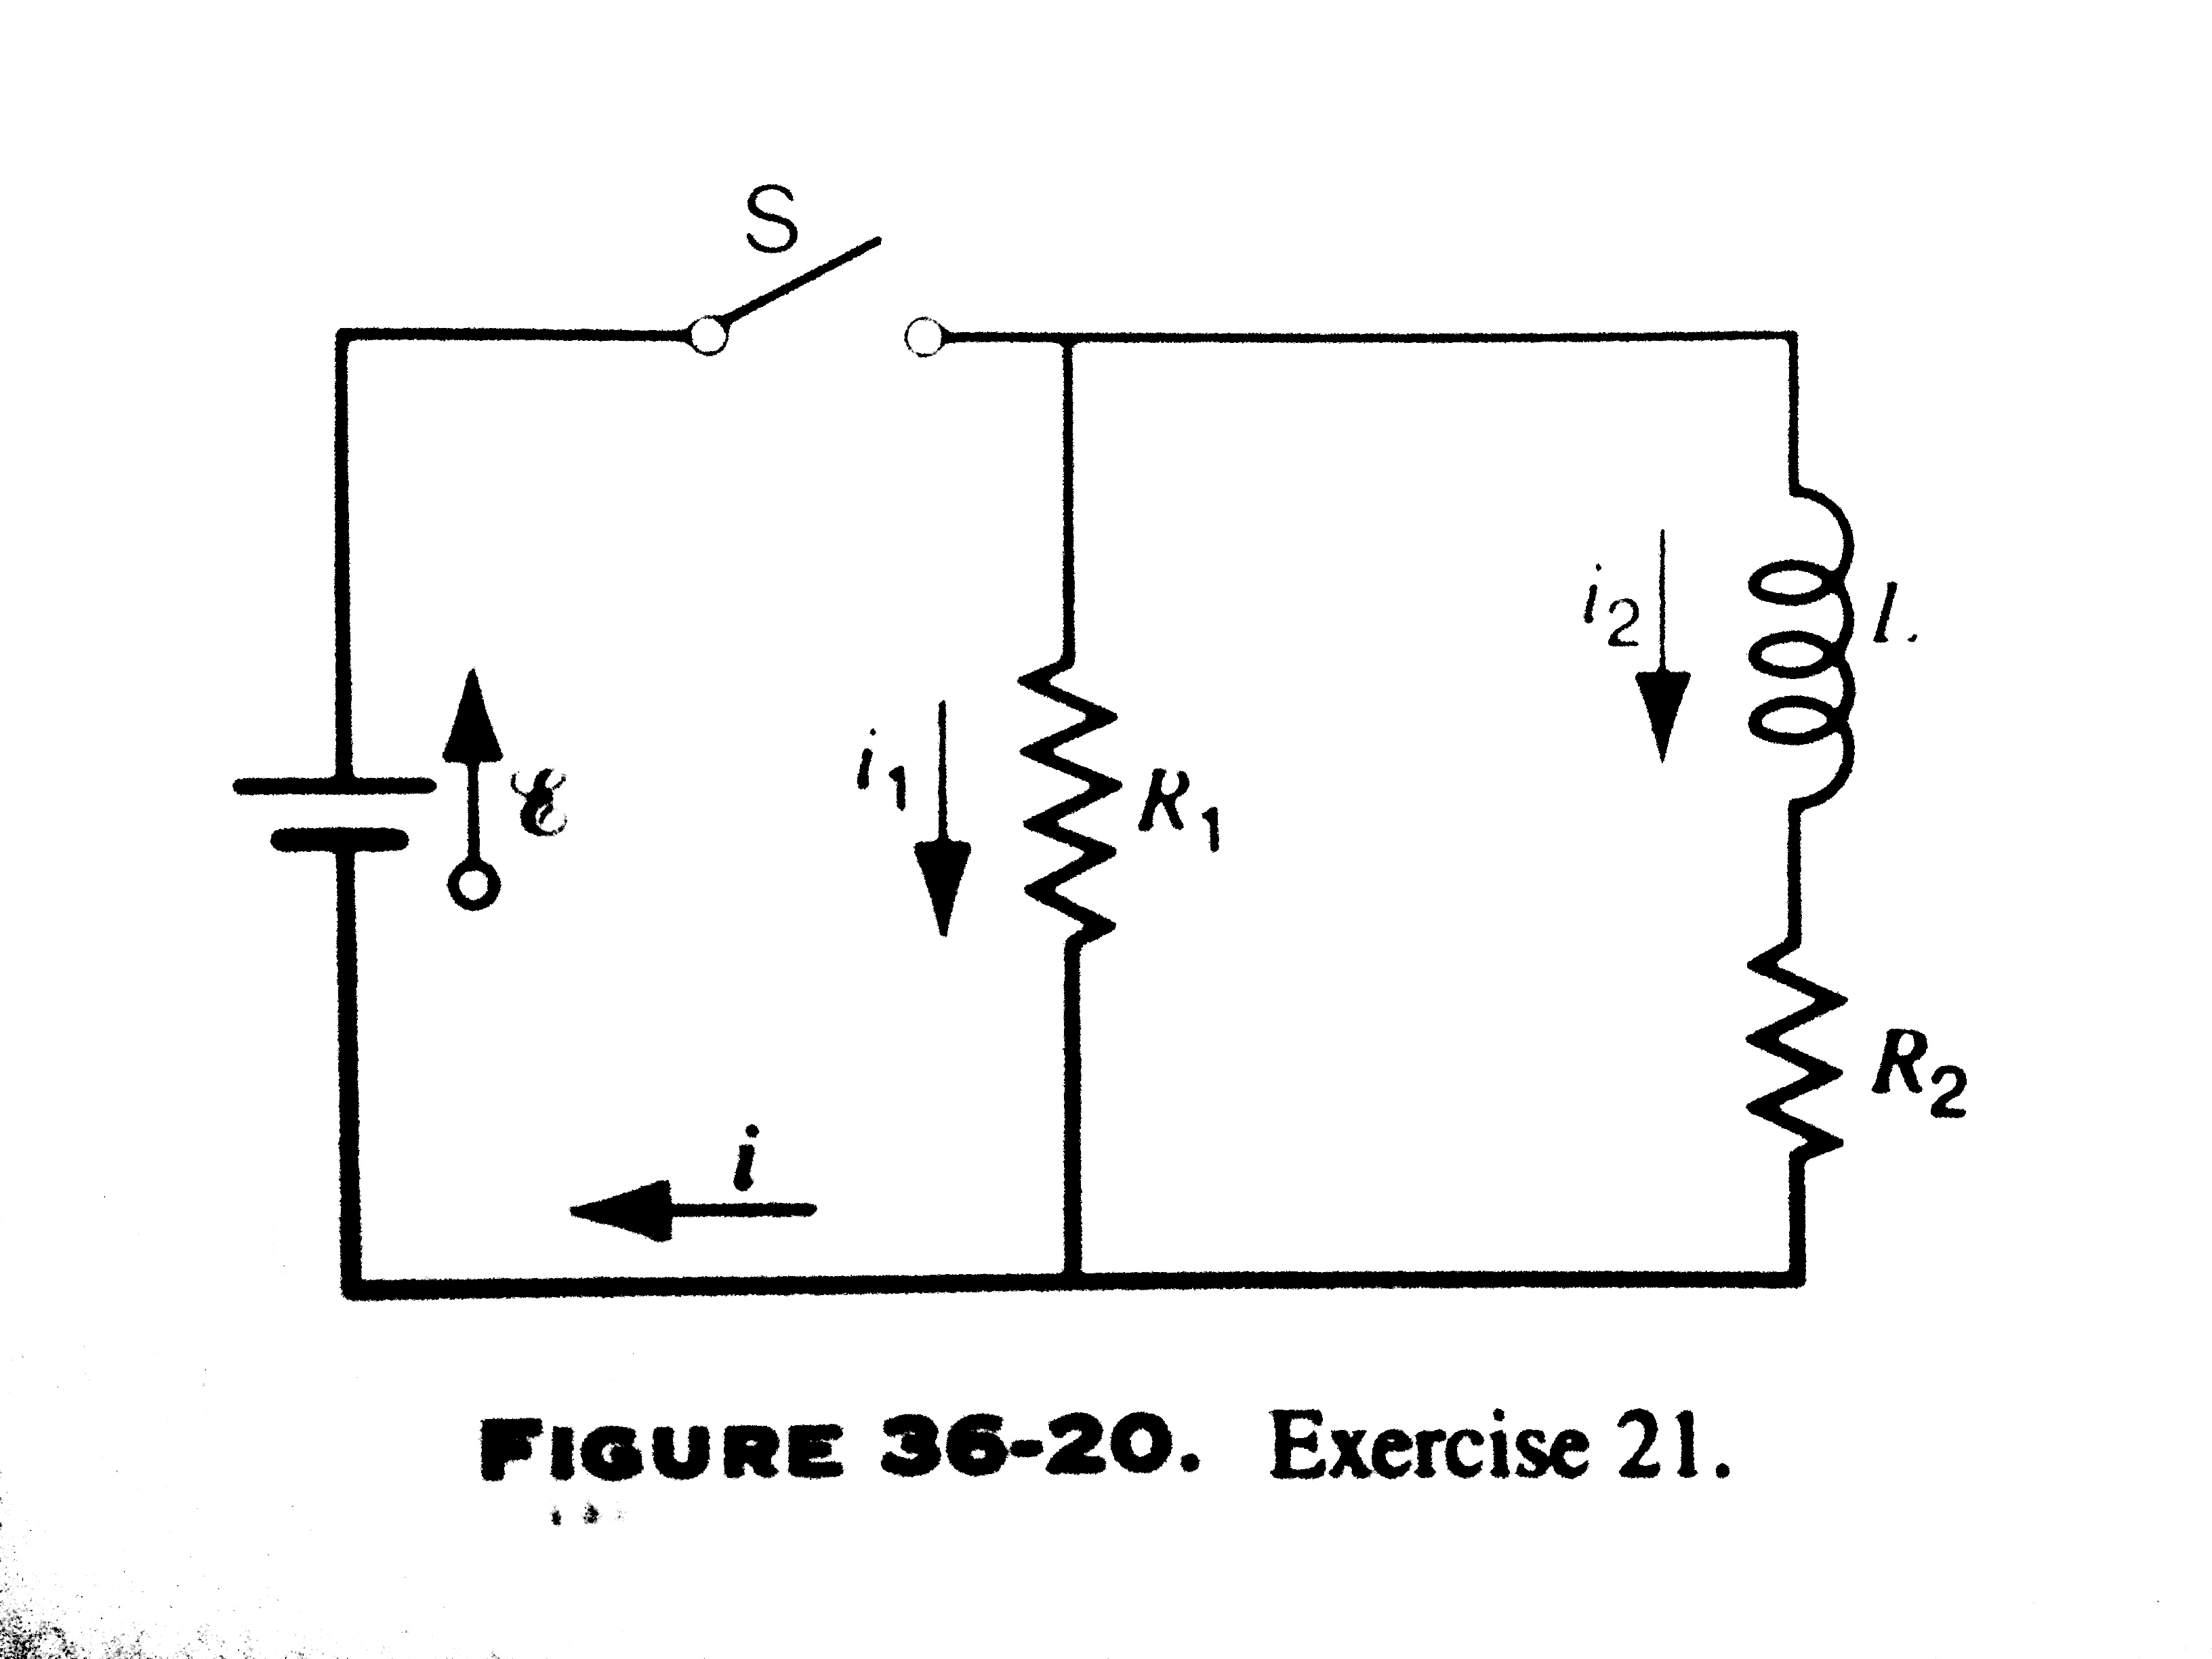
\includegraphics[scale=0.1]{01.jpg}
	\end{center}
\end{problem}
\begin{solution}
\end{solution}
\newpage


\begin{problem}[36-P9]
	\begin{enumerate}
		\item[(a)] Find an expression for the energy density as a function of the radial distance $r$ of a toroid of rectangular cross section.
		\item[(b)] Integrating the energy density over the volume of the toroid, calculate the total energy stored in the field of the toroid.
		\item[(c)] Using Eq. 36-10, evaluate the energy stored in the toroid directly from the inductance and compare with (b).
	\end{enumerate}
\end{problem}
\begin{solution}
\end{solution}


\end{document}